\documentclass[tikz]{standalone}
\usepackage{pgfplots}
\pgfplotsset{compat=1.15}
\usepackage{mathrsfs}
\usetikzlibrary{arrows,calc}
\usepackage{tkz-euclide}

\pagestyle{empty}

\definecolor{AngleClr}{rgb}{0,0.39215686274509803,0}
\definecolor{ShapeClr}{rgb}{0.6,0.2,0}

\begin{document}

\begin{tikzpicture}[scale=.75]
\tkzSetUpLine[line width=1pt,color=black]
\tkzSetUpPoint[fill=black]

\node at (0,0) {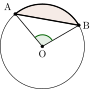
\includegraphics{circular_segment_el.pdf}};

\node[scale=4] at (3,-0.2) {$\mathbf{=}$};

\node at (6,0) {\includegraphics{circular_segment_set_diff_1_el.pdf}};

\node[scale=4] at (9,-0.2) {$\mathbf{-}$};

\node at (12,0) {\includegraphics{circular_segment_set_diff_2_el.pdf}};

\end{tikzpicture}

\end{document}
